\documentclass[a4paper,12pt]{exam}
\usepackage[a4paper]{geometry}
\usepackage{pdfpages}
\usepackage{graphicx}
\begin{document}
\pagestyle{empty}
\section*{Mixed School Problem Solving Questions}
\begin{questions}
  \question Define the “reverse” of a number to be the same digits written backwards. For example, the reverse of 135 is 531, and the reverse of 4630 is 0364. 

Prove that the sum of any four-digit number and its reverse is divisible by 11. 

Hint: Represent the 4-digit number as $ABCD$. 
    \question Suppose you have an analogue clock with an hour hand and a minute hand. If it is currently midnight, how long will it take for the two hands to form a $90^{\circ}$ angle? 

    \question How many triangles are there in the image below?
    \[  \includegraphics[scale=0.3]{how-many-triangles-do-you-see-1.png}\]

      \question 
      \begin{parts}
         \part Find the smallest integer \(x\) such that \(1800x\) is a perfect square. 
         \part What is the general strategy to find the smallest integer $x$ such that $N \times x$ is a perfect square for positive integer $N$?
      \end{parts}

      \question Why does the set of rational numbers on the interval \((0,1)\) not have a least element?

      \question
      \begin{parts}
          \part Must a quadratic pass through the $x$ axis? Why or why not?
          \part Must a cubic pass through the $x$ axis? Why or why not?
      \end{parts}

      \question  The scales at Jasper’s house only work if two people weigh themselves at
    the same time. He has four people in his house who weigh themselves in
    pairs obtaining 89kg, 105kg, 112kg, 113kg, 120kg and 136kg. What is the
    difference between the weights of the heaviest and lightest people in the
    house?

      
\end{questions}
  

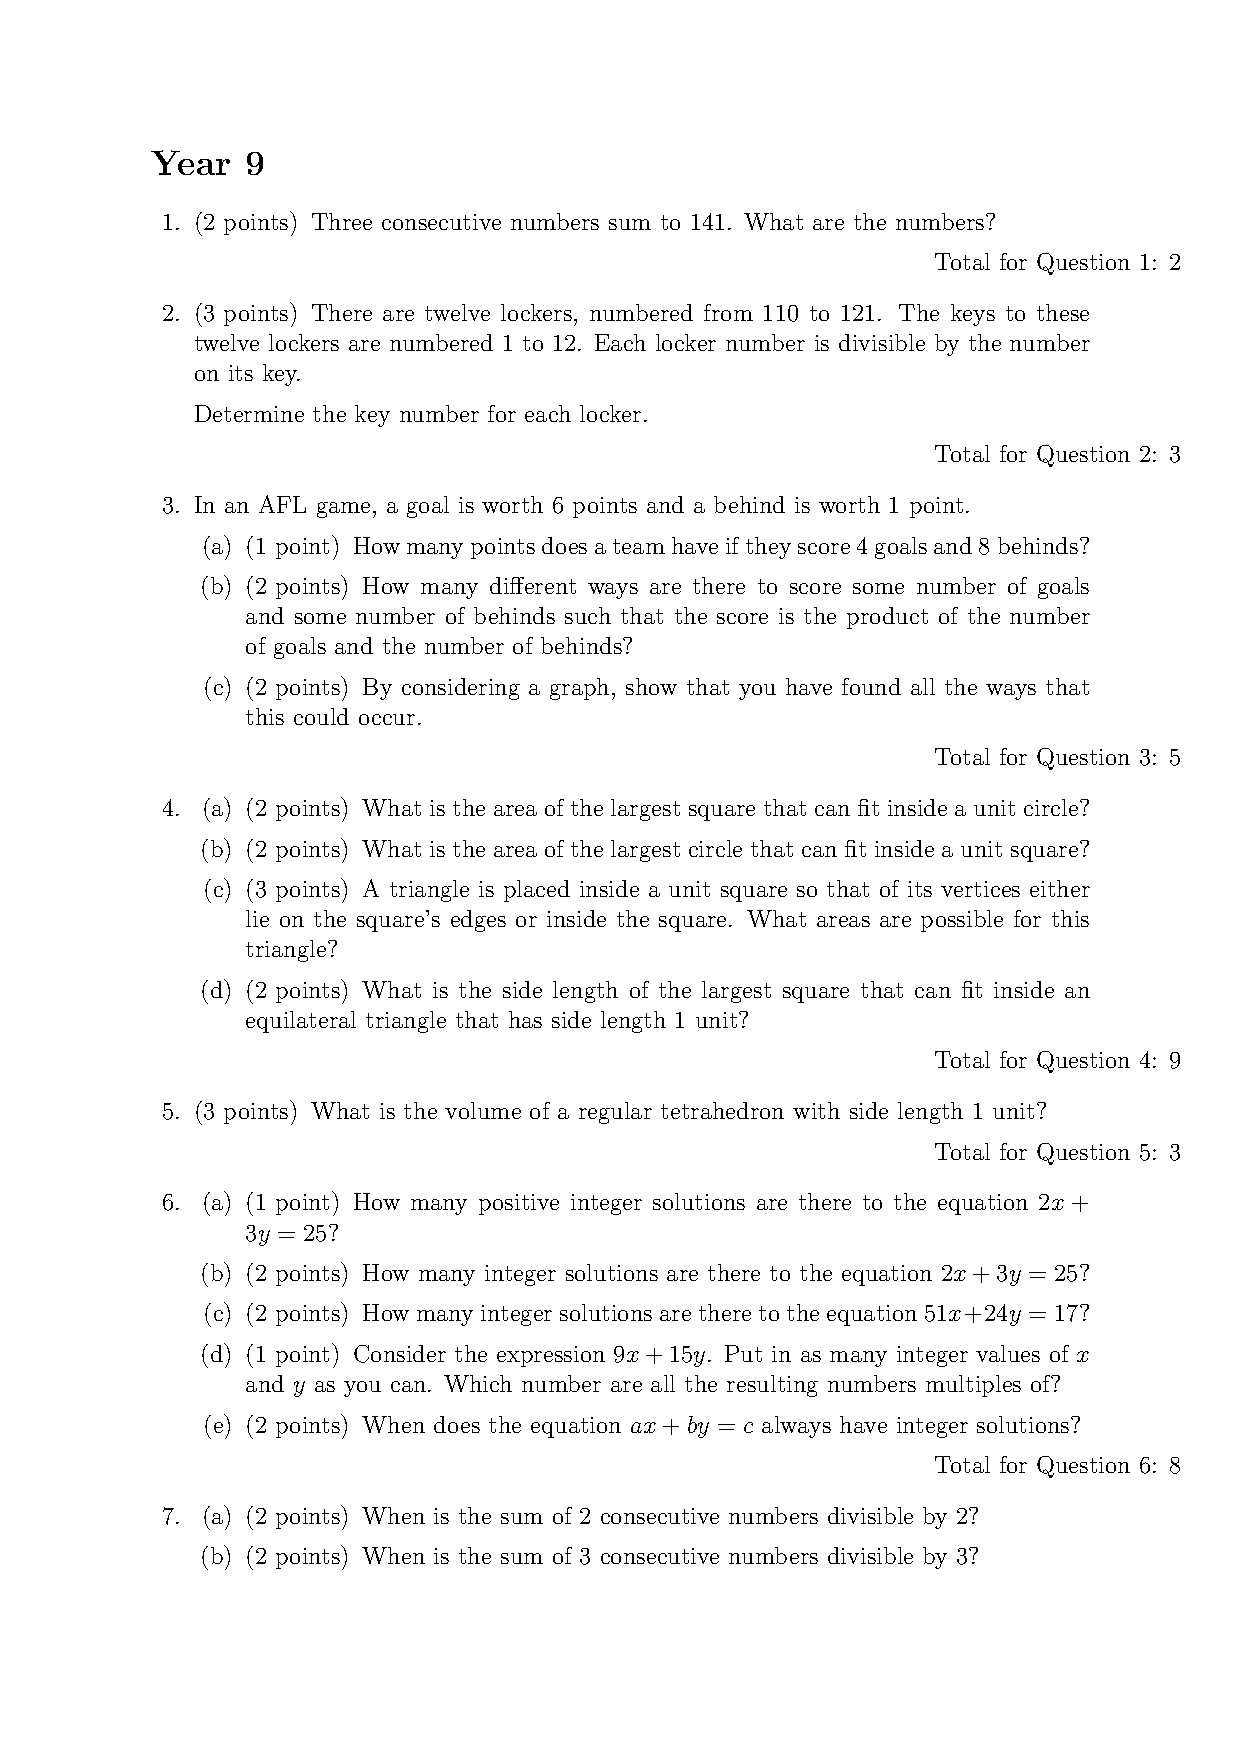
\includepdf[pages=-]{SEHS_Maths_Games_Day_2023_Problem_Solving_Year9}
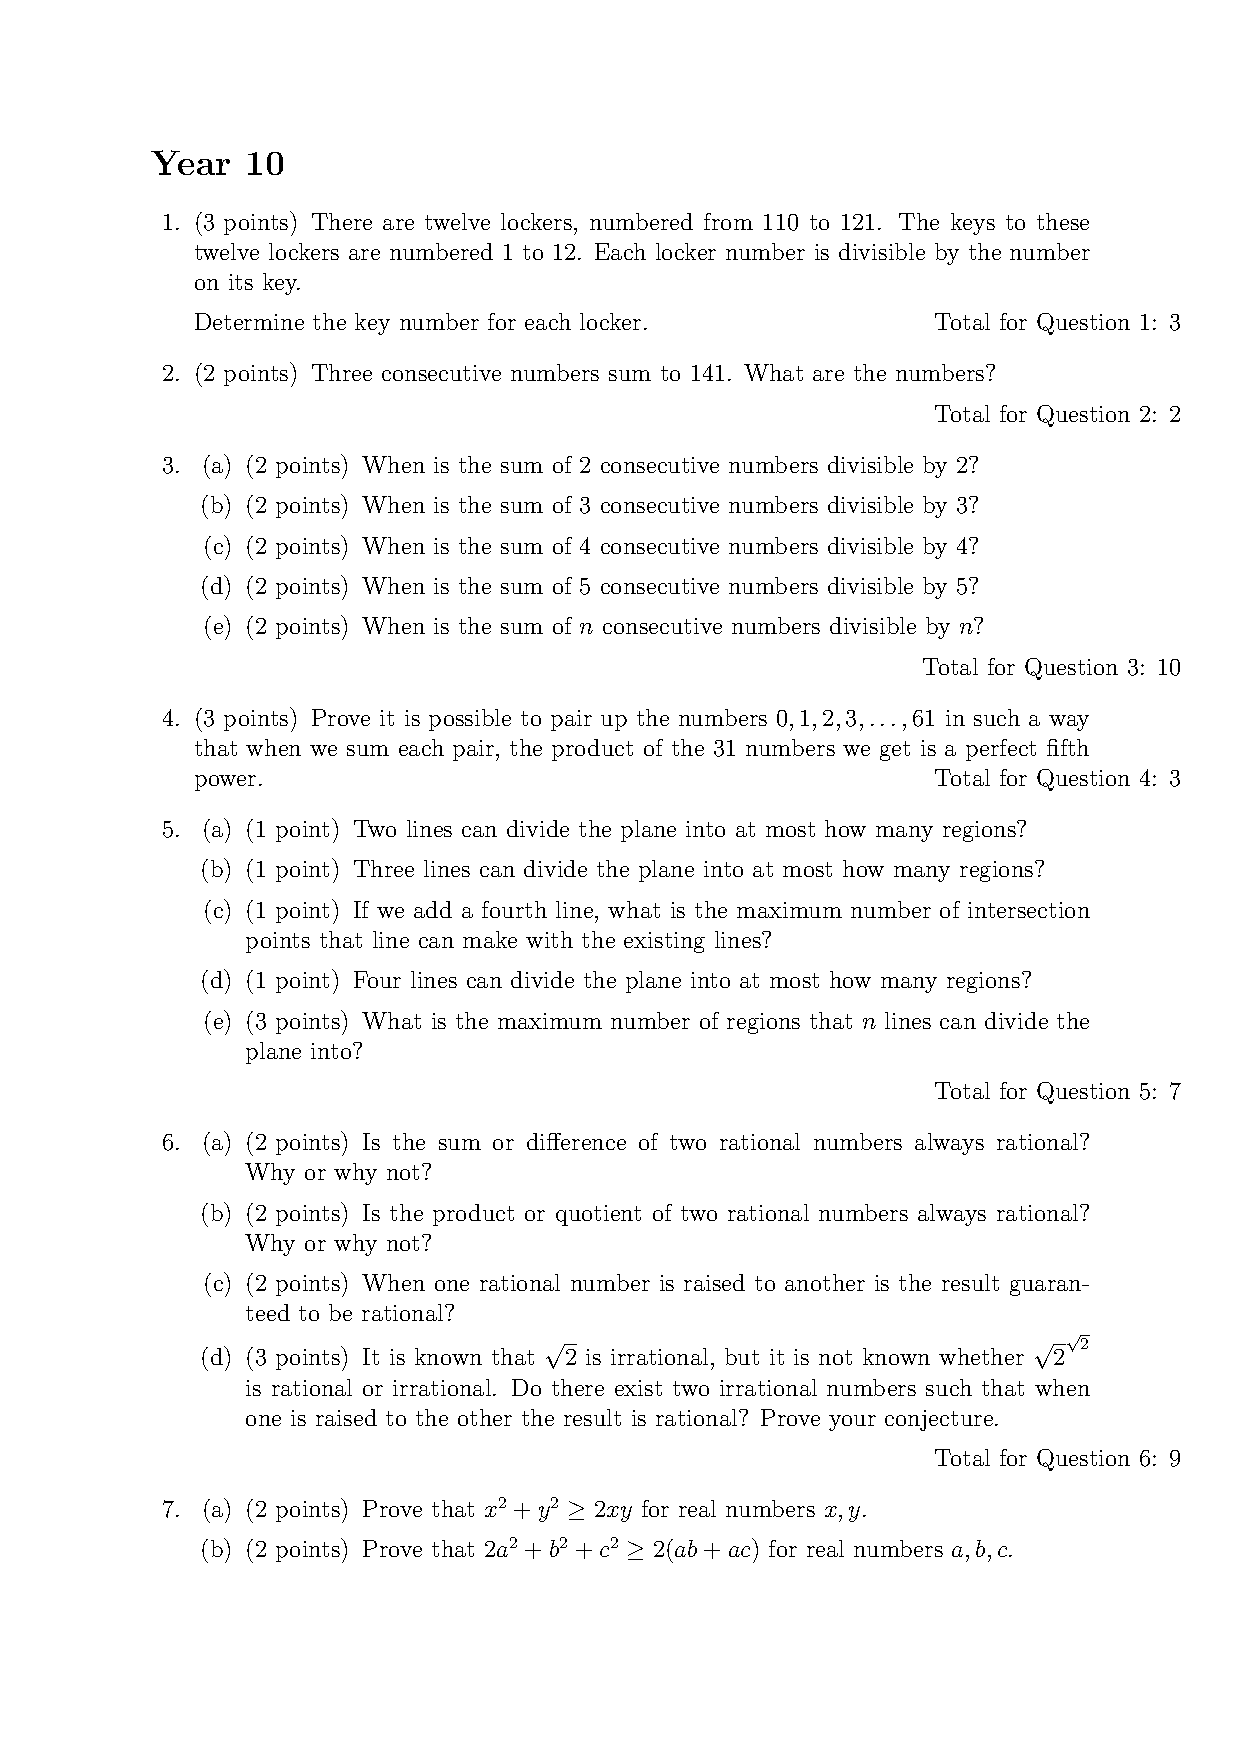
\includepdf[pages=-]{SEHS_Maths_Games_Day_2023_Problem_Solving_Year10}
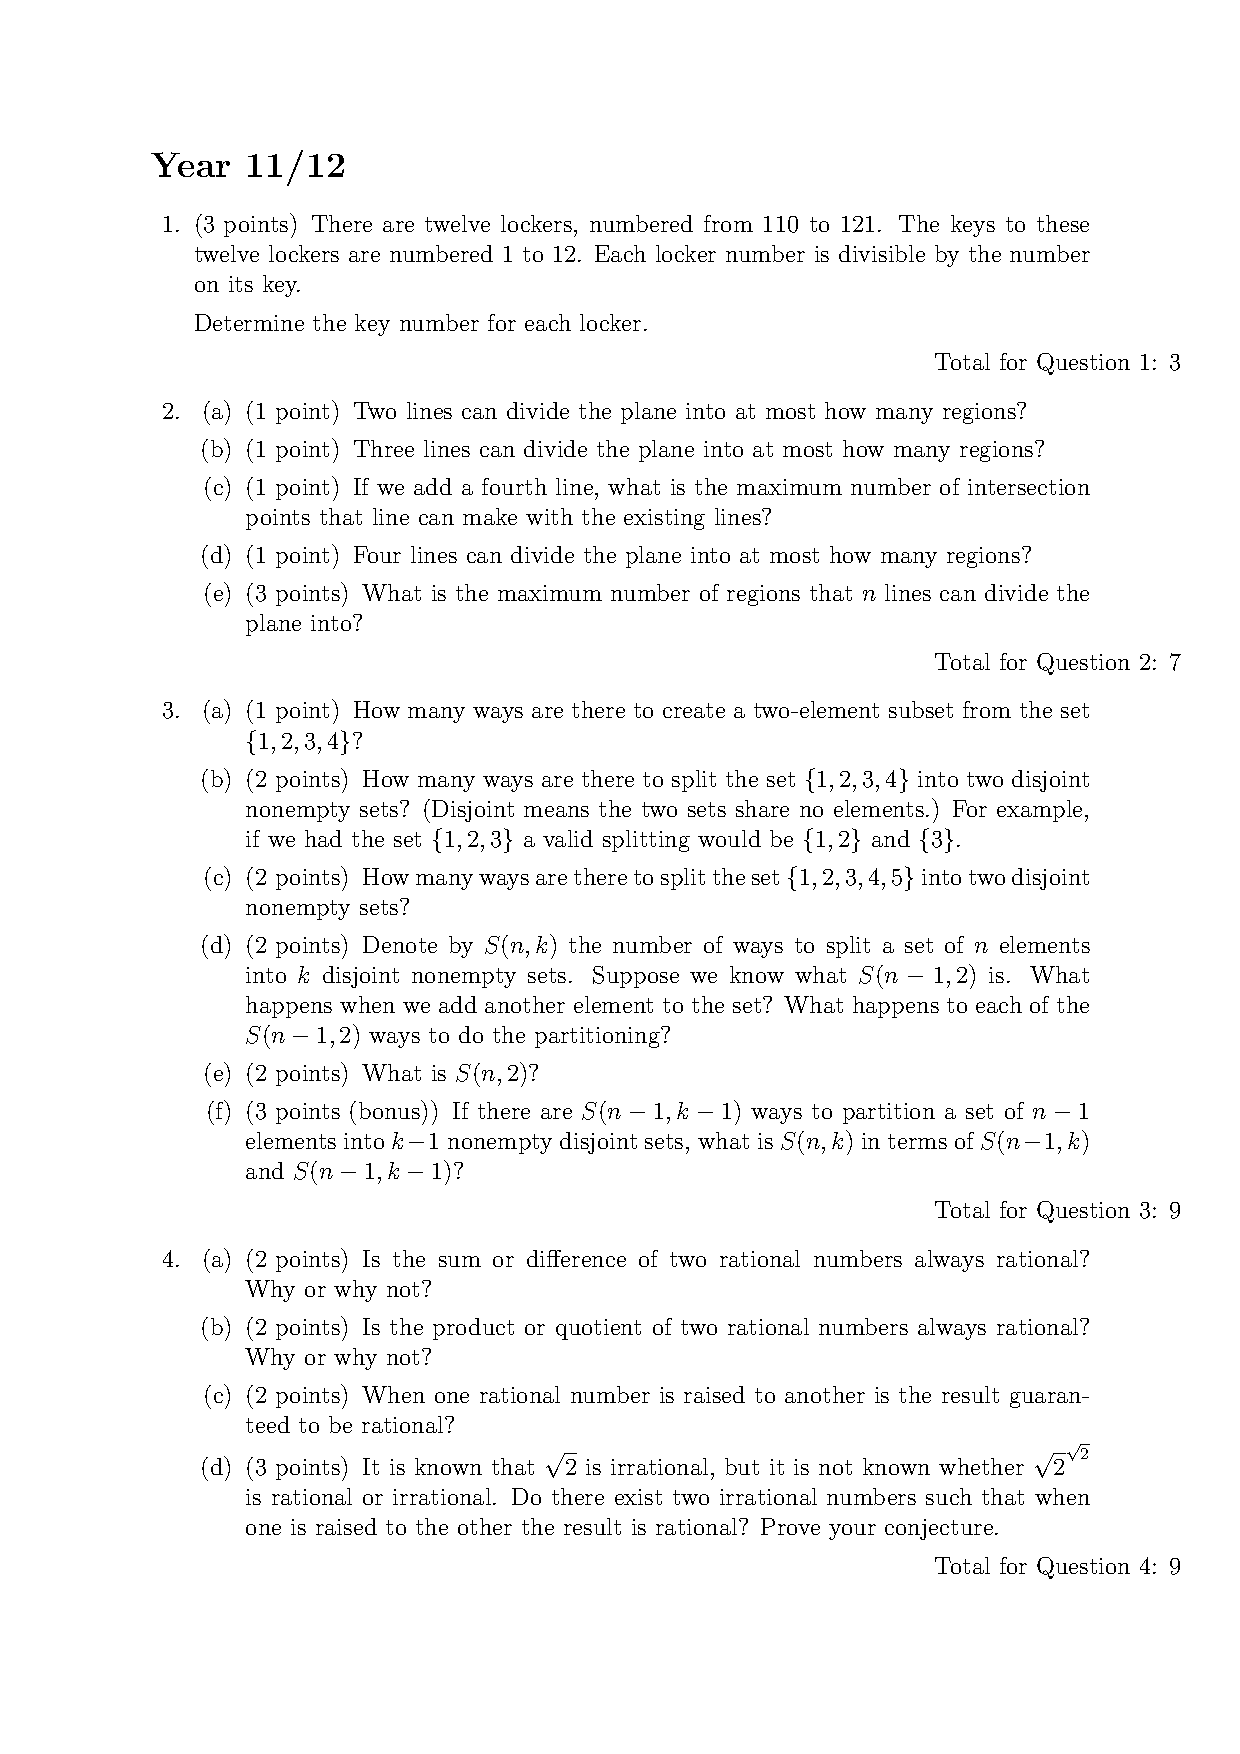
\includepdf[pages=-]{SEHS_Maths_Games_Day_2023_Problem_Solving_Year11-12}
\end{document}